%%%%%%%%%%%%%%%%%%%%%%%%%%%%%%%%%%%
%% Uso de la clase ITTol-Tesis
%%%%%%%%%%%%%%%%%%%%%%%%%%%%%%%%%%%
\documentclass[12pt]{ITTol-Tesis}

% Paquete usado para incluir texto falso (Lorem Ipsum) en el ejemplo 
\usepackage{lipsum}					

% Para links sin decoración
%\hypersetup{colorlinks=false,allbordercolors=white}

\titulo{Título de la Tesis}
\autor{Autor de la Tesis}
\grado{Maestro en Ciencias en Ciencias de la Ingeniería}
\date{Octubre de 2018}
\director{Director de la Tesis}
\codirector{Codirector de la Tesis}                                      % Si existe un codirector
%\tutor{Tutor}                                                                      % Si existe un tutor
\autorizacion{autoImpresionTesis}                               	% Oficio de autorización de impresión de Tesis (png, pdf, jpg) 
\aprobacion{dictamenAprobacionTesis} 				% Dictamen de aprobación de Tesis por la comisión revisora
											% (png, pdf, jpg)

%%%%%%%%%%%%%%%%%%%%%%%%%%%%%%%%%%%
%% Documento
%%%%%%%%%%%%%%%%%%%%%%%%%%%%%%%%%%%
\begin{document}

\maketitle	                                                                            % Crea la carátula
\frontmatter

\insertarautorizacion                                                            % Autorización
\insertaraprobacion                                                              % Aprobación

%%%%%%%%%%%%%%%%%%%%%%%%%%%%%%%%%%%
%% Dedicatoria
\begin{dedicatoria}                                                              
\begin{center}
Escriba aquí su dedicatoria.
\end{center}
\end{dedicatoria}

%%%%%%%%%%%%%%%%%%%%%%%%%%%%%%%%%%%
%% Resumen en español
\begin{abstract}                                                                   
\textcolor{gray}{Se presentará en forma breve los aspectos relevantes de su Tesis, como objetivos, 
resultados y posibles aplicaciones.  No deberá exceder a una cuartilla.}\\

\lipsum[1]
\end{abstract}


%%%%%%%%%%%%%%%%%%%%%%%%%%%%%%%%%%%
%% Resumen en inglés
\selectlanguage{english}                                                     
\begin{abstract}
\textcolor{gray}{The relevant aspects of your thesis will be briefly presented, such as objectives,
results and possible applications. It should not exceed one page.}\\

\lipsum[1]
\end{abstract}


%%%%%%%%%%%%%%%%%%%%%%%%%%%%%%%%%%%
%% Agradecimientos
\selectlanguage{spanish}
\begin{agradecimientos}                                                     
\begin{center}
\textbf{AGRADECIMIENTOS}
\end{center}
\lipsum[1-3]
\end{agradecimientos}


%%%%%%%%%%%%%%%%%%%%%%%%%%%%%%%%%%%
%% Índices
\tableofcontents                                                                   % Índice de Contenido
{\noskip\listoffigures}                                                            % Índice de Figuras
{\noskip\listoftables}                                                             % Índice de Tablas

\mainmatter

%%%%%%%%%%%%%%%%%%%%%%%%%%%%%%%%%%%
%% Capítulos
%%%%%%%%%%%%%%%%%%%%%%%%%%%%%%%%%%%%%%%%%%%%%%%%%%%%%%%%%%%%
%% Capítulo 1 / Introducción
%%%%%%%%%%%%%%%%%%%%%%%%%%%%%%%%%%%%%%%%%%%%%%%%%%%%%%%%%%%%
\chapter{Introducción}
\epigrafe{Everyone in this country should learn how to program a computer, because it teaches you how to think.}
              {\textsc{Steve Jobs}}

\textcolor{gray}{Es el contenido global de lo que va a encontrarse en el trabajo. Incluye los aspectos relevantes de los antecedentes, la definición del problema, la justificación, los objetivos: general y específicos. En este apartado se iniciará la paginación principal con números arábigos (los capítulos podrán ir numerados con arábigos)}

%%%%%%%%%%%%%%%%%%%%%%%%%%%%%%%%%%%%%%%%%%%%%%%%%%%%%%%%%%%%
\section{Ejemplo Figura}
\lipsum[1] 
Como se puede apreciar en la Figura \ref{fig:01_Proceso}.

\begin{figure}[htbp]                                                      % Inclusión de una figura
\centering
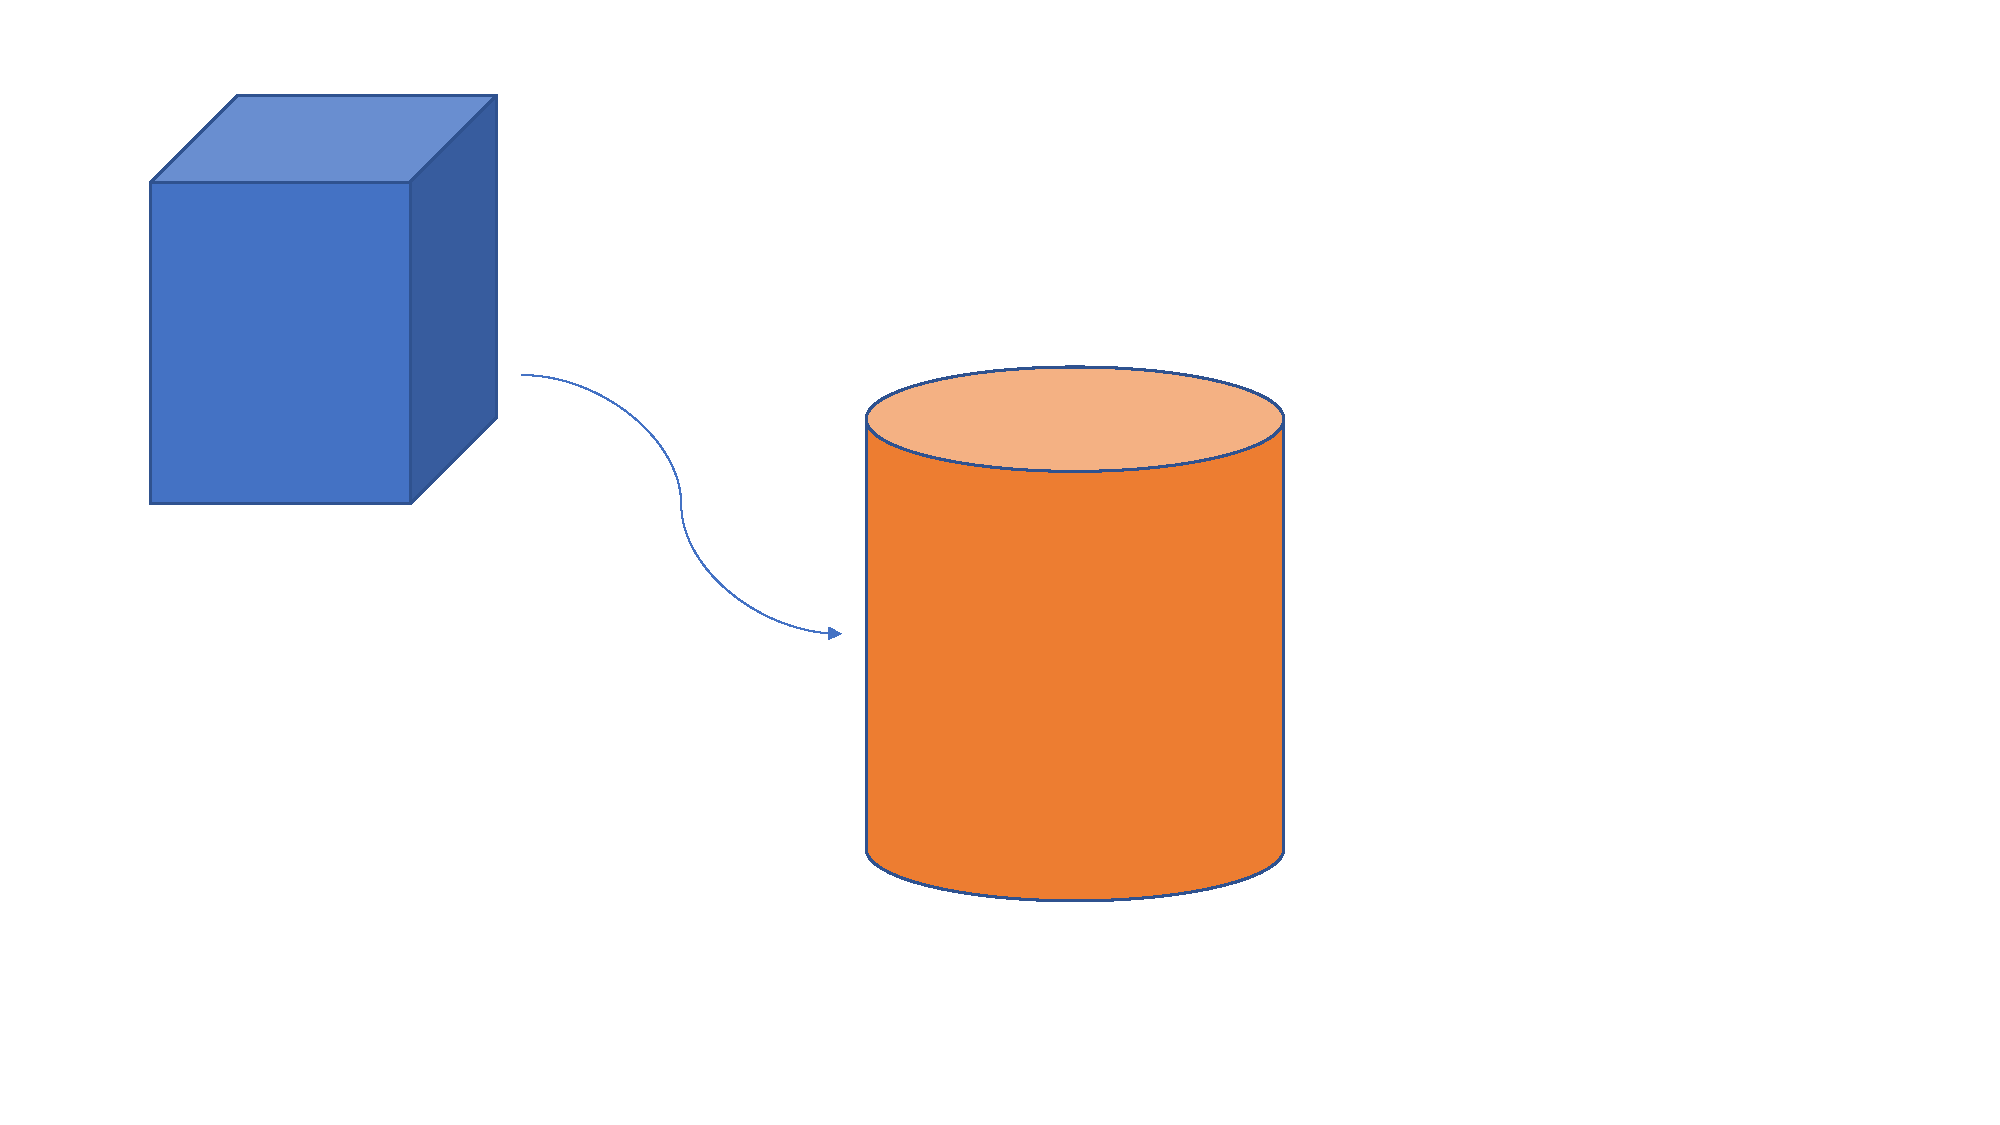
\includegraphics[width=0.80\textwidth]{a_Imagen01}
\caption{Donec vehicula augue eu neque.}
\label{fig:01_Proceso}
\end{figure}

\lipsum[2]


%%%%%%%%%%%%%%%%%%%%%%%%%%%%%%%%%%%%%%%%%%%%%%%%%%%%%%%%%%%%
\section{Ejemplo Link}
\lipsum[3-4]
En el \href{https://es.wikipedia.org/wiki/Proceso_(ingenier%C3%ADa)}{Wikipedia - Proceso} se pueden consultar la descripción
del proceso mostrado en la Figura~\ref{fig:01_Proceso}. 
                                                      % Introducción.tex
%%%%%%%%%%%%%%%%%%%%%%%%%%%%%%%%%%%%%%%%%%%%%%%%%%%%%%%%%%%%
%% Capítulo 2 / Fundamentos Teóricos y Problemática
%%%%%%%%%%%%%%%%%%%%%%%%%%%%%%%%%%%%%%%%%%%%%%%%%%%%%%%%%%%%
\chapter{Fundamentos Teóricos y Problemática}
\epigrafe{Everyone in this country should learn how to program a computer, because it teaches you how to think.}
              {\textsc{Steve Jobs}}
              
\textcolor{gray}{Es esencial abordar en este apartado el conocimiento existente acerca del tema que se desarrolla. Los puntos a desarrollar son los siguientes: El contexto en el que se desarrolla el trabajo; la teoría en la que se fundamenta; el estado del arte, que se refiere a la recopilación de toda la información relevante, que a la fecha exista, relacionada con la temática. }

\section{Ejemplo Ecuación}

\lipsum[1]

\begin{equation}                                                     
\mathrm{e}^{x} = \sum_{k=0}^{\infty} \frac{x^k}{k!} = 
1 + x + \frac{x^2}{2} + \frac{x^3}{6} + \cdots
\label{eq:taylor}
\end{equation}

La ecuación \eqref{eq:taylor} muestra la expansión en serie de Taylor alrededor de $x = 0$ para la función exponencial natural.

\section{Ejemplo Cita Bibliográfica}
\lipsum[3-4].  
Los fundamentos también pueden revisarse en \cite{knuth97}. 

\section{Tercera sección}
\lipsum[5-6]
                     		                 % Fundamento.tex
%%%%%%%%%%%%%%%%%%%%%%%%%%%%%%%%%%%%%%%%%%%%%%%%%%%%%%%%%%%%
%% Capítulo 4 / Metodología
%%%%%%%%%%%%%%%%%%%%%%%%%%%%%%%%%%%%%%%%%%%%%%%%%%%%%%%%%%%%
\chapter{Metodología}
\epigrafe{Everyone in this country should learn how to program a computer, because it teaches you how to think.}
              {\textsc{Steve Jobs}}
              
\textcolor{gray}{En este apartado se explican los pasos que se desarrollaron, en cada una de las etapas del trabajo de tesis, se debe tener cuidado de ser congruente. Si es necesario, apoyarse con un esquema a fin de mostrar de manera global el desarrollo del trabajo e ir presentando posteriormente la descripción de cada una de las etapas.}

\section{Primera sección}
\lipsum[1-2]. 
Se deben atender las recomendaciones y buena prácticas indicadas en su seminario de investigación, de tesis, o de
las referencias bibliográficas pertinentes, por ejemplo \cite{Sampieri}. 

\section{Ejemplo Algoritmo}
\lipsum[3]
\lipsum[4].
El análisis de datos se realiza con el Algoritmo \ref{Alg:Algo-01}, descrito en seguida:

\begin{algorithm}[H]
  \SetAlgoLined
  \KwData{this text}
  \KwResult{how to write algorithm with \LaTeX2e }
  initialization\;
  \While{not at end of this document}{
    read current\;
    \eIf{understand}{
      go to next section\;
      current section becomes this one\;
      }{
      go back to the beginning of current section\;
      }
    }
  \caption{How to write algorithms}
  \label{Alg:Algo-01}
\end{algorithm}

\section{Ejemplos Citas Bibliográficas}
\lipsum[1-2].
Actualmente existen las siguiente propuestas de \cite{lopez2013impacto} y \cite{orduna2016revolucion}.


                                                      % Metodología
%%%%%%%%%%%%%%%%%%%%%%%%%%%%%%%%%%%%%%%%%%%%%%%%%%%%%%%%%%%%
%% Capítulo 5 / Resultados
%%%%%%%%%%%%%%%%%%%%%%%%%%%%%%%%%%%%%%%%%%%%%%%%%%%%%%%%%%%%
\chapter{Resultados y discusión}
\epigrafe{Everyone in this country should learn how to program a computer, because it teaches you how to think.}
              {\textsc{Steve Jobs}}


\textcolor{gray}{Explicar detallamente los logros obtenidos acorde a los objetivos planteados y que sean concordantes con la hipótesis propuesta. Discutir los hallazgos considerando referencias relacionadas con el 
tema de estudio.}

\section{Ejemplo Tabla}
\lipsum[1].  
Los resultados pueden verse en la Tabla \ref{tab:Tabla1}

\begin{table}[htbp]
\centering
\caption{Resultados obtenidos.}
\label{tab:pversust}
\begin{tabular}{ccc}
\toprule
\textbf{Parametro A } & \textbf{Resultado } \\
\midrule
A & 1 \\
B & 2 \\ 
C & 3 \\
D & 4 \\
\bottomrule
\end{tabular}
\label{tab:Tabla1}
\end{table}

\lipsum[2]

\section{Ejemplo Figura}
\lipsum[3-4]

\begin{figure}[htbp]
\centering
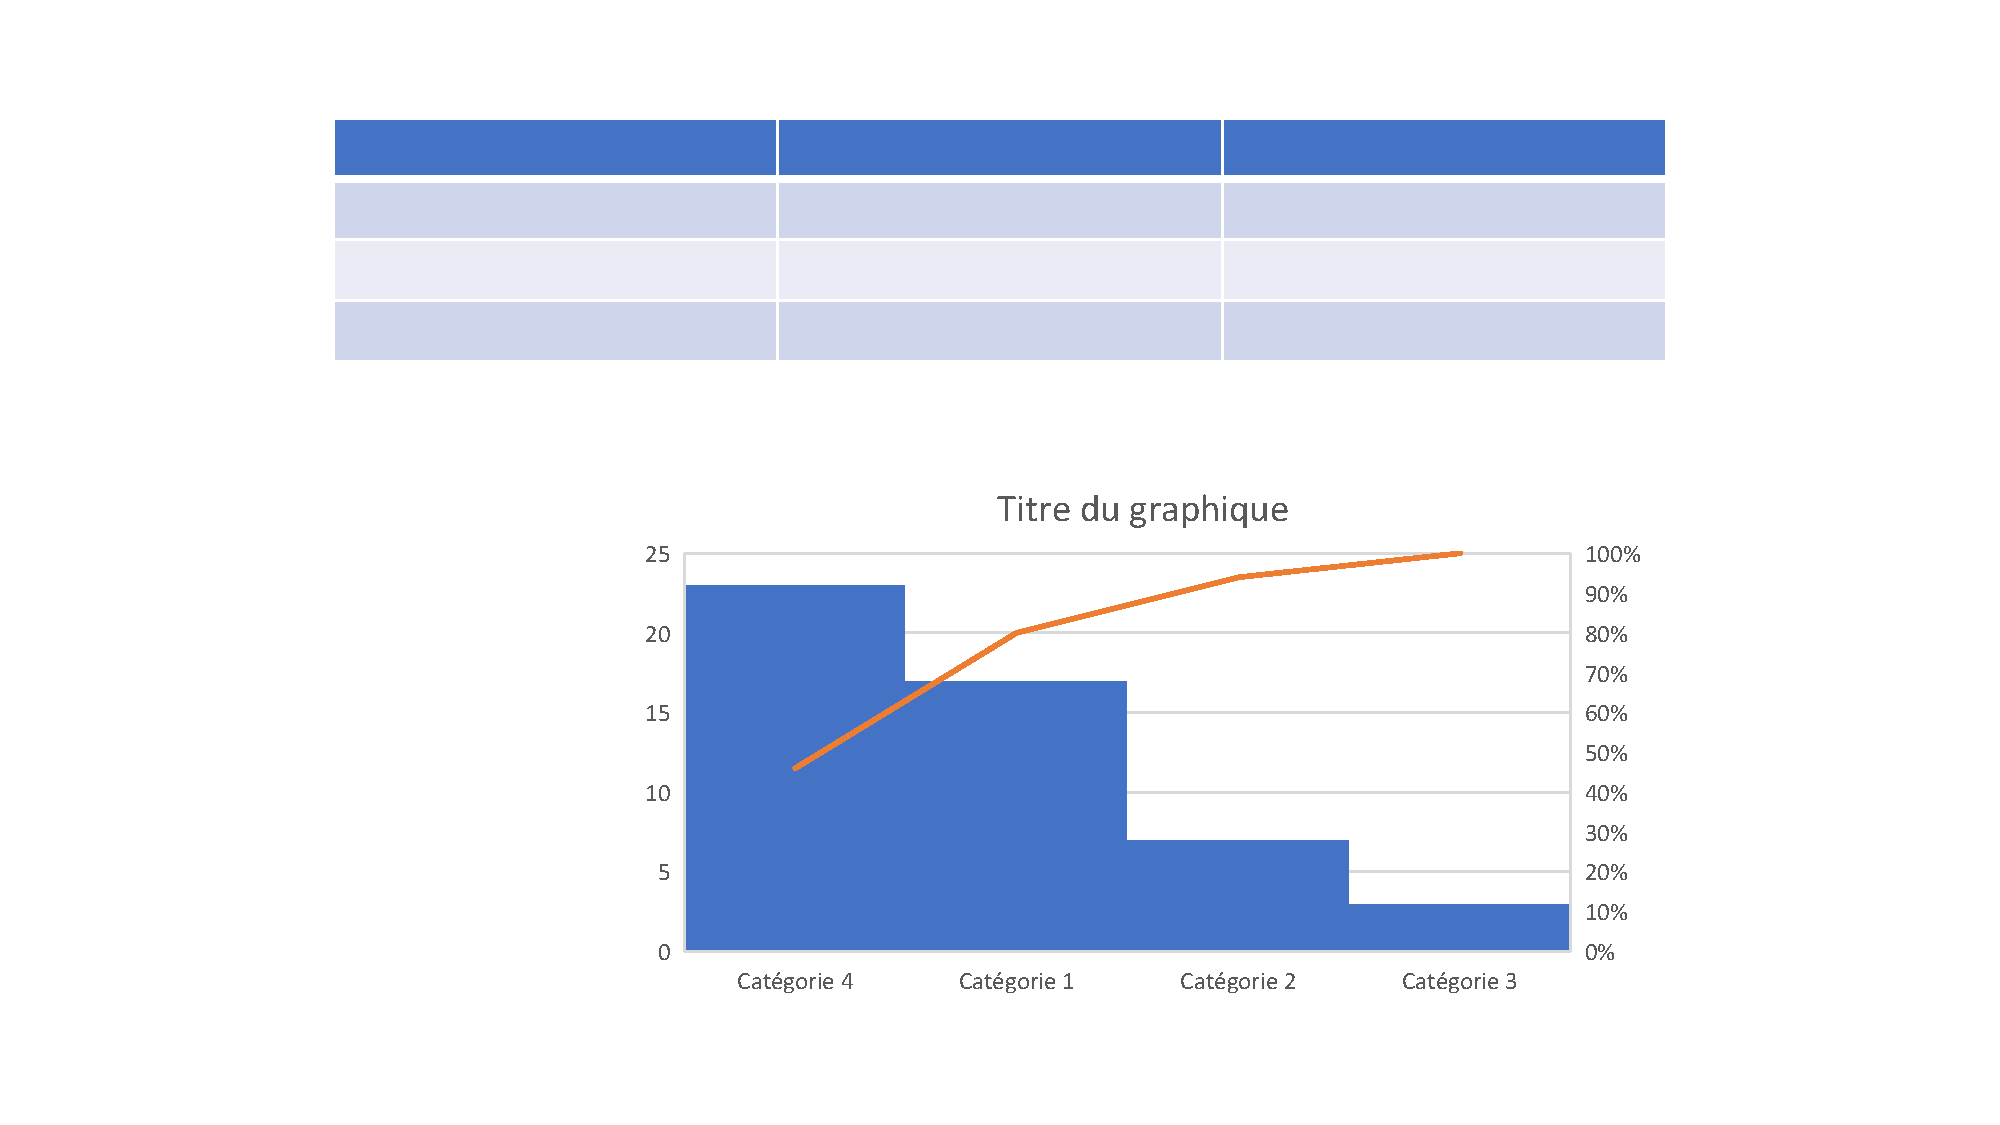
\includegraphics[width=0.50\textwidth]{e_Imagen01}
\caption{Duis eget orci sit amet orci dignissim rutrum.}
\label{fig:particion}
\end{figure}

\section{Tercera sección}
\lipsum[5-6]
                                                       % Resultados
%%%%%%%%%%%%%%%%%%%%%%%%%%%%%%%%%%%%%%%%%%%%%%%%%%%%%%%%%%%%
%% Capítulo 6 / Conclusiones y Perspectivas
%%%%%%%%%%%%%%%%%%%%%%%%%%%%%%%%%%%%%%%%%%%%%%%%%%%%%%%%%%%%
\chapter{Conclusiones y recomendaciones}
\epigrafe{Everyone in this country should learn how to program a computer, because it teaches you how to think.}
              {\textsc{Steve Jobs}}
              
\textcolor{gray}{Concluir únicamente con los resultados obtenidos de la investigación de acuerdo a los objetivos y a la verificación de la hipótesis. Es importante comentar que este apartado no se debe de considerar como un resumen de resultados. Mencionar las recomendaciones que se consideren pertinentes, de acuerdo con las experiencias obtenidas, dentro del desarrollo del trabajo de tesis. Evitar los párrafos largos y las frases con varias ideas ( 6 a 7 renglones)}              

\section{Conclusiones}
\lipsum[1-3]

\section{Perspectivas}
\lipsum[1]							% Conclusiones, Perspectivas

%%%%%%%%%%%%%%%%%%%%%%%%%%%%%%%%%%%
%% Apéndices o Anexos (Opcionales)
\appendix	
%%%%%%%%%%%%%%%%%%%%%%%%%%%%%%%%%%%%%%%%%%%%%%%%%%%%%%%%%%%%
%% Apéndice A / Demostraciones
%%%%%%%%%%%%%%%%%%%%%%%%%%%%%%%%%%%%%%%%%%%%%%%%%%%%%%%%%%%%
\chapter{Demostraciones}

\section{Explicando Teorema}
\lipsum[1-2].

\begin{proof} 
  Esta es mi demostración $a \times (b+c)=a \times b + a \times c$ 
\end{proof}
			         % Demostraciones
%%%%%%%%%%%%%%%%%%%%%%%%%%%%%%%%%%%%%%%%%%%%%%%%%%%%%%%%%%%%
%% Apéndice B / Código Fuente
%%%%%%%%%%%%%%%%%%%%%%%%%%%%%%%%%%%%%%%%%%%%%%%%%%%%%%%%%%%%

%%%%%%%%%%%%%%%%%%%%%%%%%%%%%%%%%%%%%%%%%%%%%%%%%%%%% Preparación para el paquete listing
\definecolor{gray97}{gray}{.97}
\definecolor{gray75}{gray}{.75}
\definecolor{gray45}{gray}{.45}

\lstset{ frame=Ltb,
  framerule=0pt,
  aboveskip=0.5cm,
  framextopmargin=3pt,
  framexbottommargin=3pt,
  framexleftmargin=0.4cm,
  framesep=0pt,
  rulesep=.4pt,
  backgroundcolor=\color{gray97},
  rulesepcolor=\color{black},
  %
  stringstyle=\ttfamily,
  showstringspaces = false,
  basicstyle=\small\ttfamily,
  commentstyle=\color{gray45},
  keywordstyle=\bfseries,
  %
  numbers=left,
  numbersep=15pt,
  numberstyle=\tiny,
  numberfirstline = false,
  breaklines=true,
}
% Personalizando los ambientes para listing
\lstnewenvironment{listing}[1][]{
  \lstset{#1}\pagebreak[0]
}
{\pagebreak[0]}
\lstdefinestyle{terminal}{			% Terminal
  basicstyle=\scriptsize\bf\ttfamily,
  backgroundcolor=\color{gray75},
}
\lstdefinestyle{C} {				% Código en C
  language=C,
}

%%%%%%%%%%%%%%%%%%%%%%%%%%%%%%%%%%%%%%%%%%%%%%%%%%%%%%%%%%%%
\chapter{Código Fuente}

\section{Explicando un programa}
\lipsum[1-2]

\noindent
Escribe el siguiente programa en un archivo llamado \texttt{hola.c}:

\begin{lstlisting}[style=C]
#include <stdio.h>

int main(int argc, char* argv[]) 
{
    printf("Hola mundo!");
}
\end{lstlisting}

\noindent
Ahora compila usando \texttt{gcc}:

\begin{listing}[style=terminal, numbers=none]
$ gcc  -o hola hola.c
\end{listing}			          	  	 % Diagramas

\backmatter

%% Bibliografía
%%%%%%%%%%%%%%%%%%%%%%%%%%%%%%%%%%%
\bibliographystyle{apacite}
\bibliography{biblio}								% Archivo .bib
\nocite{*}

\end{document}